\section{Benötigte Bauteile}

Folgend nicht inkludiert sind Bauteile welche nicht als projektspezifisch anzusehen sind, sowie Rohmaterialien.

Alle für den Versuchsaufbau verwendeten Komponenten werden in Teil 6 unter dem Punkt \hyperref[labuebung]{\textit{Laborübung}} nochmals detailliert beschrieben.
Dort ist auch ihr konkreter Verwendungszweck exakter ausgeführt.

\begin{itemize}
    \item Halbbrücken-Wägezelle 50kg
    \item Vollbrücken-Wägezelle 5kg
    \item IR-Sensor
    \item HX-711
    \item Arduino Nano
    \item Rohrschelle
    \item Bremsscheibe
\end{itemize}

\subsection{Wägezellen}

Die ursprünglich verwendete 50 Kilogramm Wägezelle wurde im Laufe der Arbeit mit einer Vollbrücken-Wägezelle, welche eine Maximallast von 5 Kilogramm hat ausgetauscht.
Dies wurde als sinnvoll erachtet, da diese über einen ausreichenden Bereich funktionsfähig ist, sowie geringere Fehler liefert.

Eine konkrete Auswahl konnte erst nach ermitteln der im Zuge des Versuches maximalen Last getroffen werden.
Trotz der schlechteren Erfüllung der Anforderungen wurde eine 5kg anstatt einer 2kg Variante gewählt, da zweitere bei keinem Anbieter auf Lager war.

Zwei auf der Wägezelle platzierte DMS (Dehnungsmessstreifen) verändern bei Biegen des Federkörpers ihren Wiederstand minimal, wodurch auch die abfallende Spannung sich verändert.

\begin{figure}[H]
    \centering
    \hfill
    \subfigure[Halbbrücken Wägezelle 50kg]{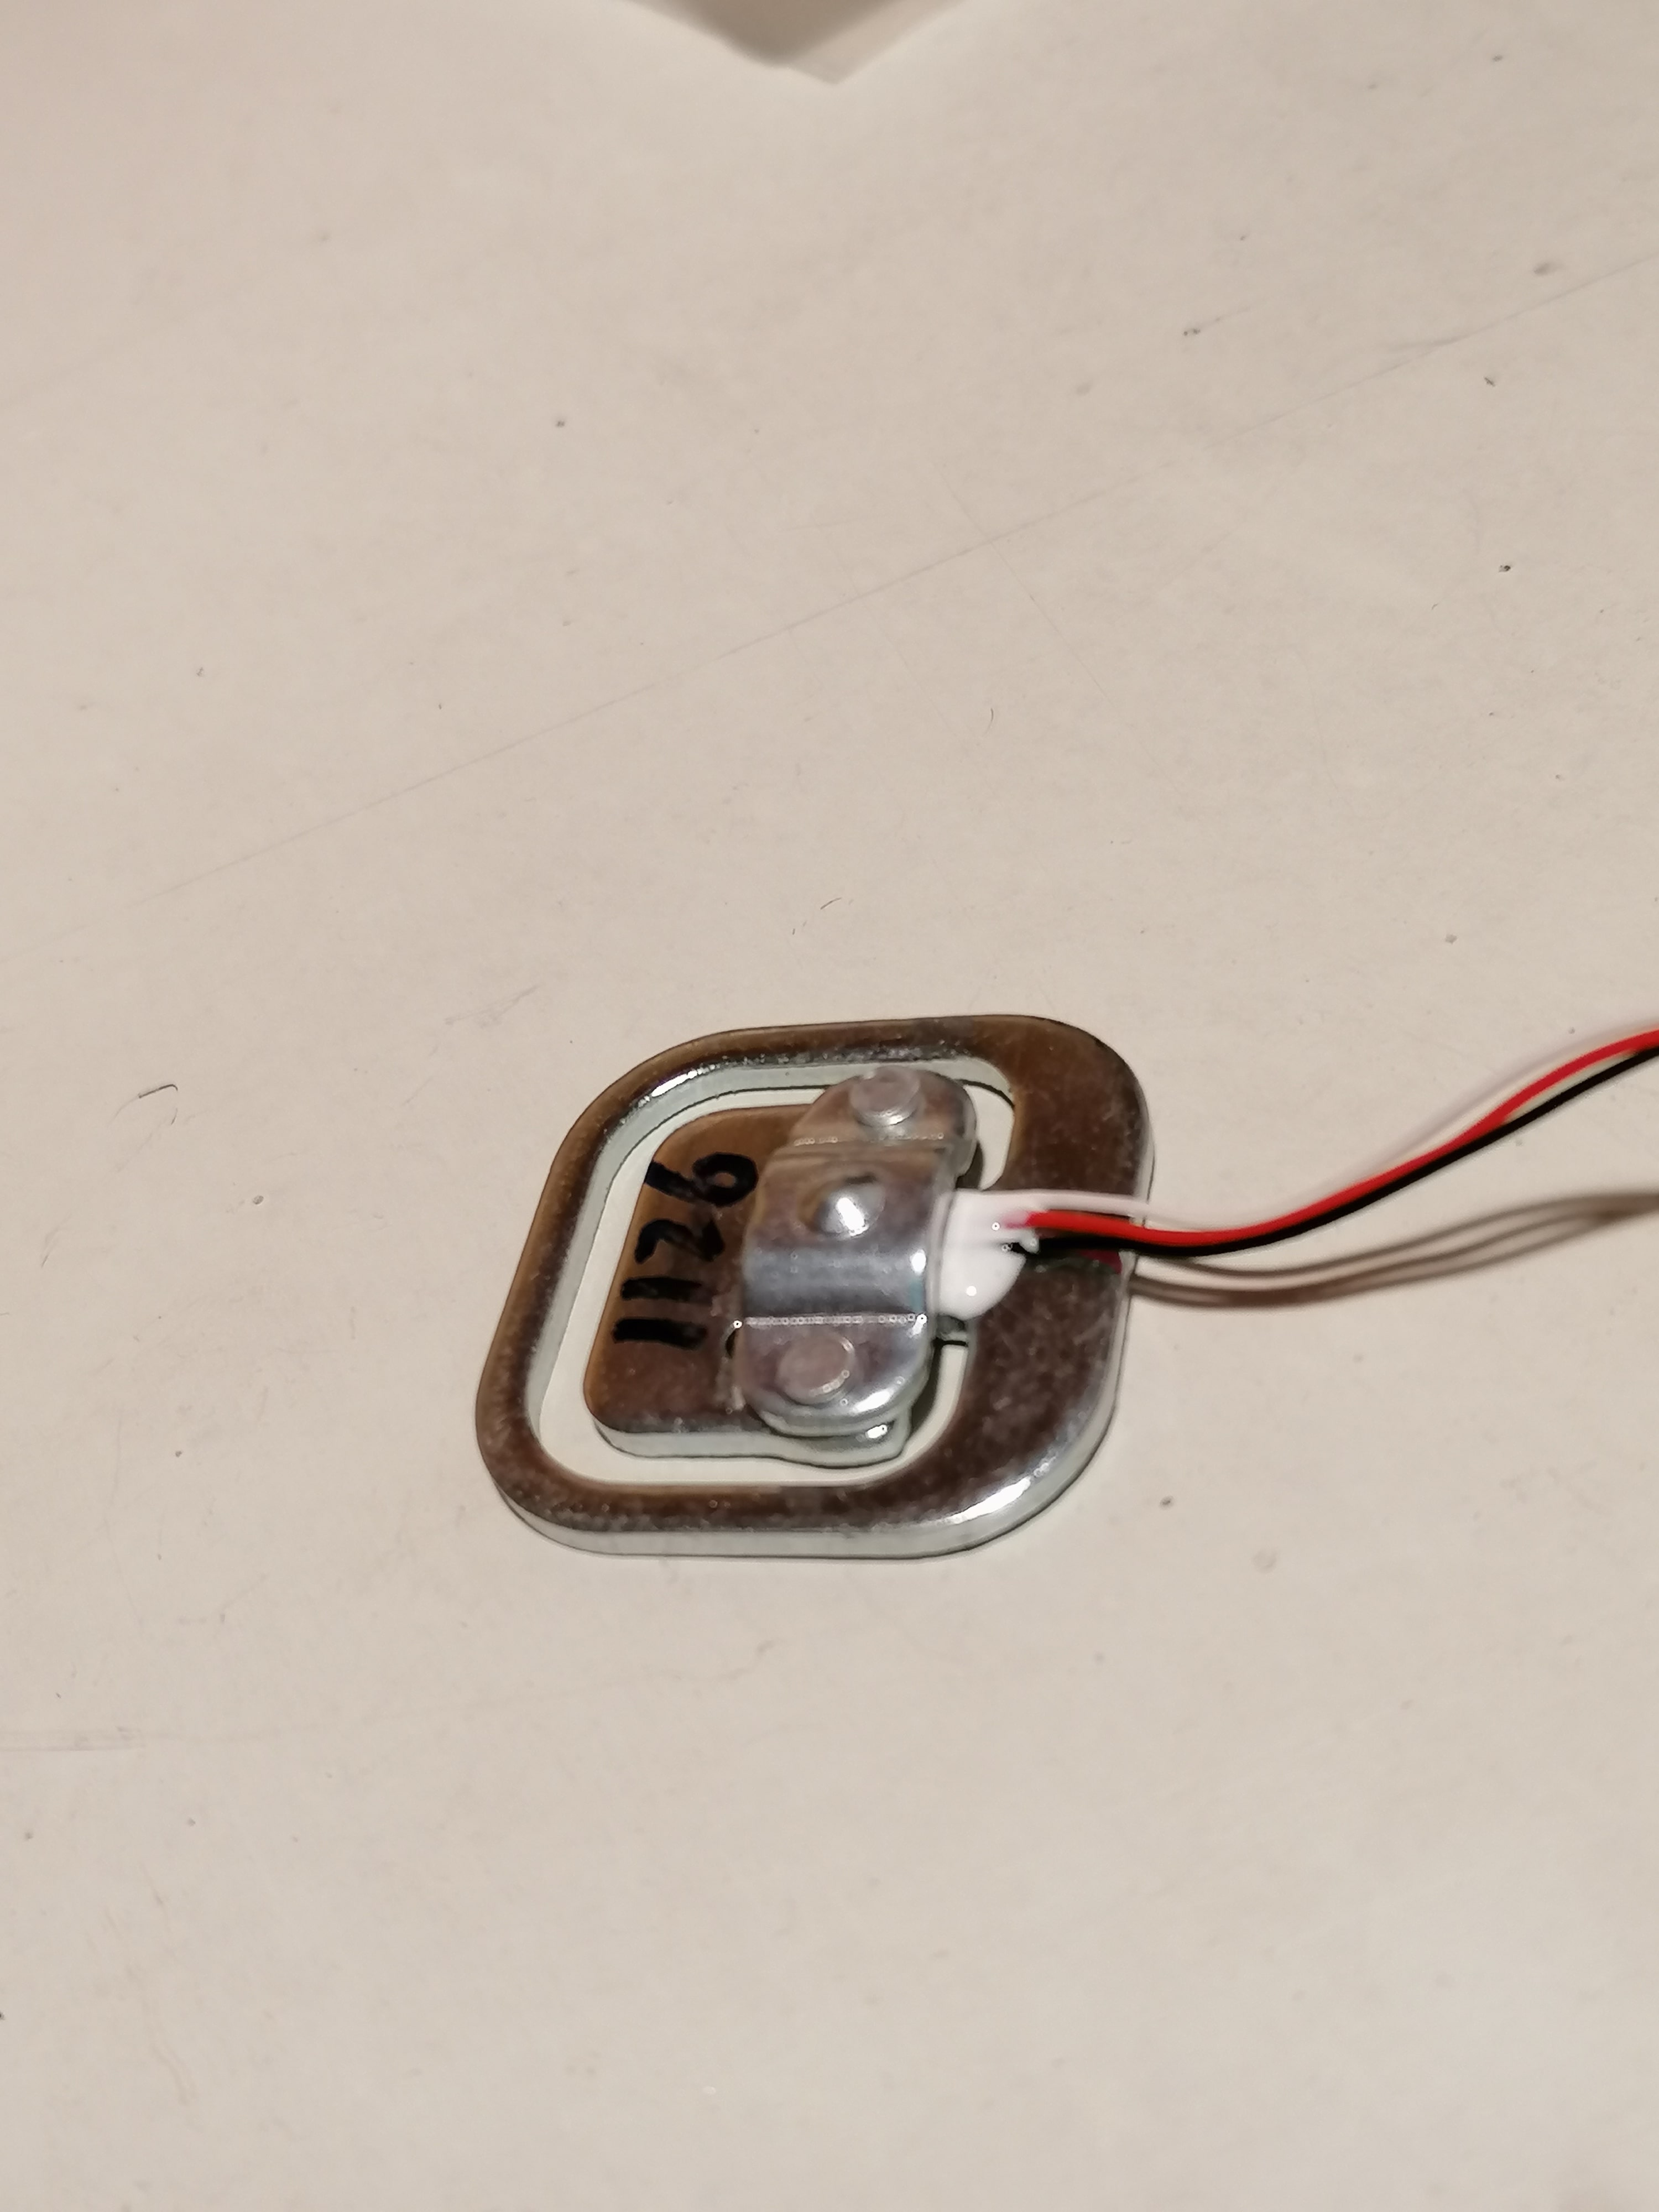
\includegraphics[width=0.3\textwidth]{waegezelle2.jpg}}
    \hfill
    \subfigure[Vollbrücken Wägezelle 5kg]{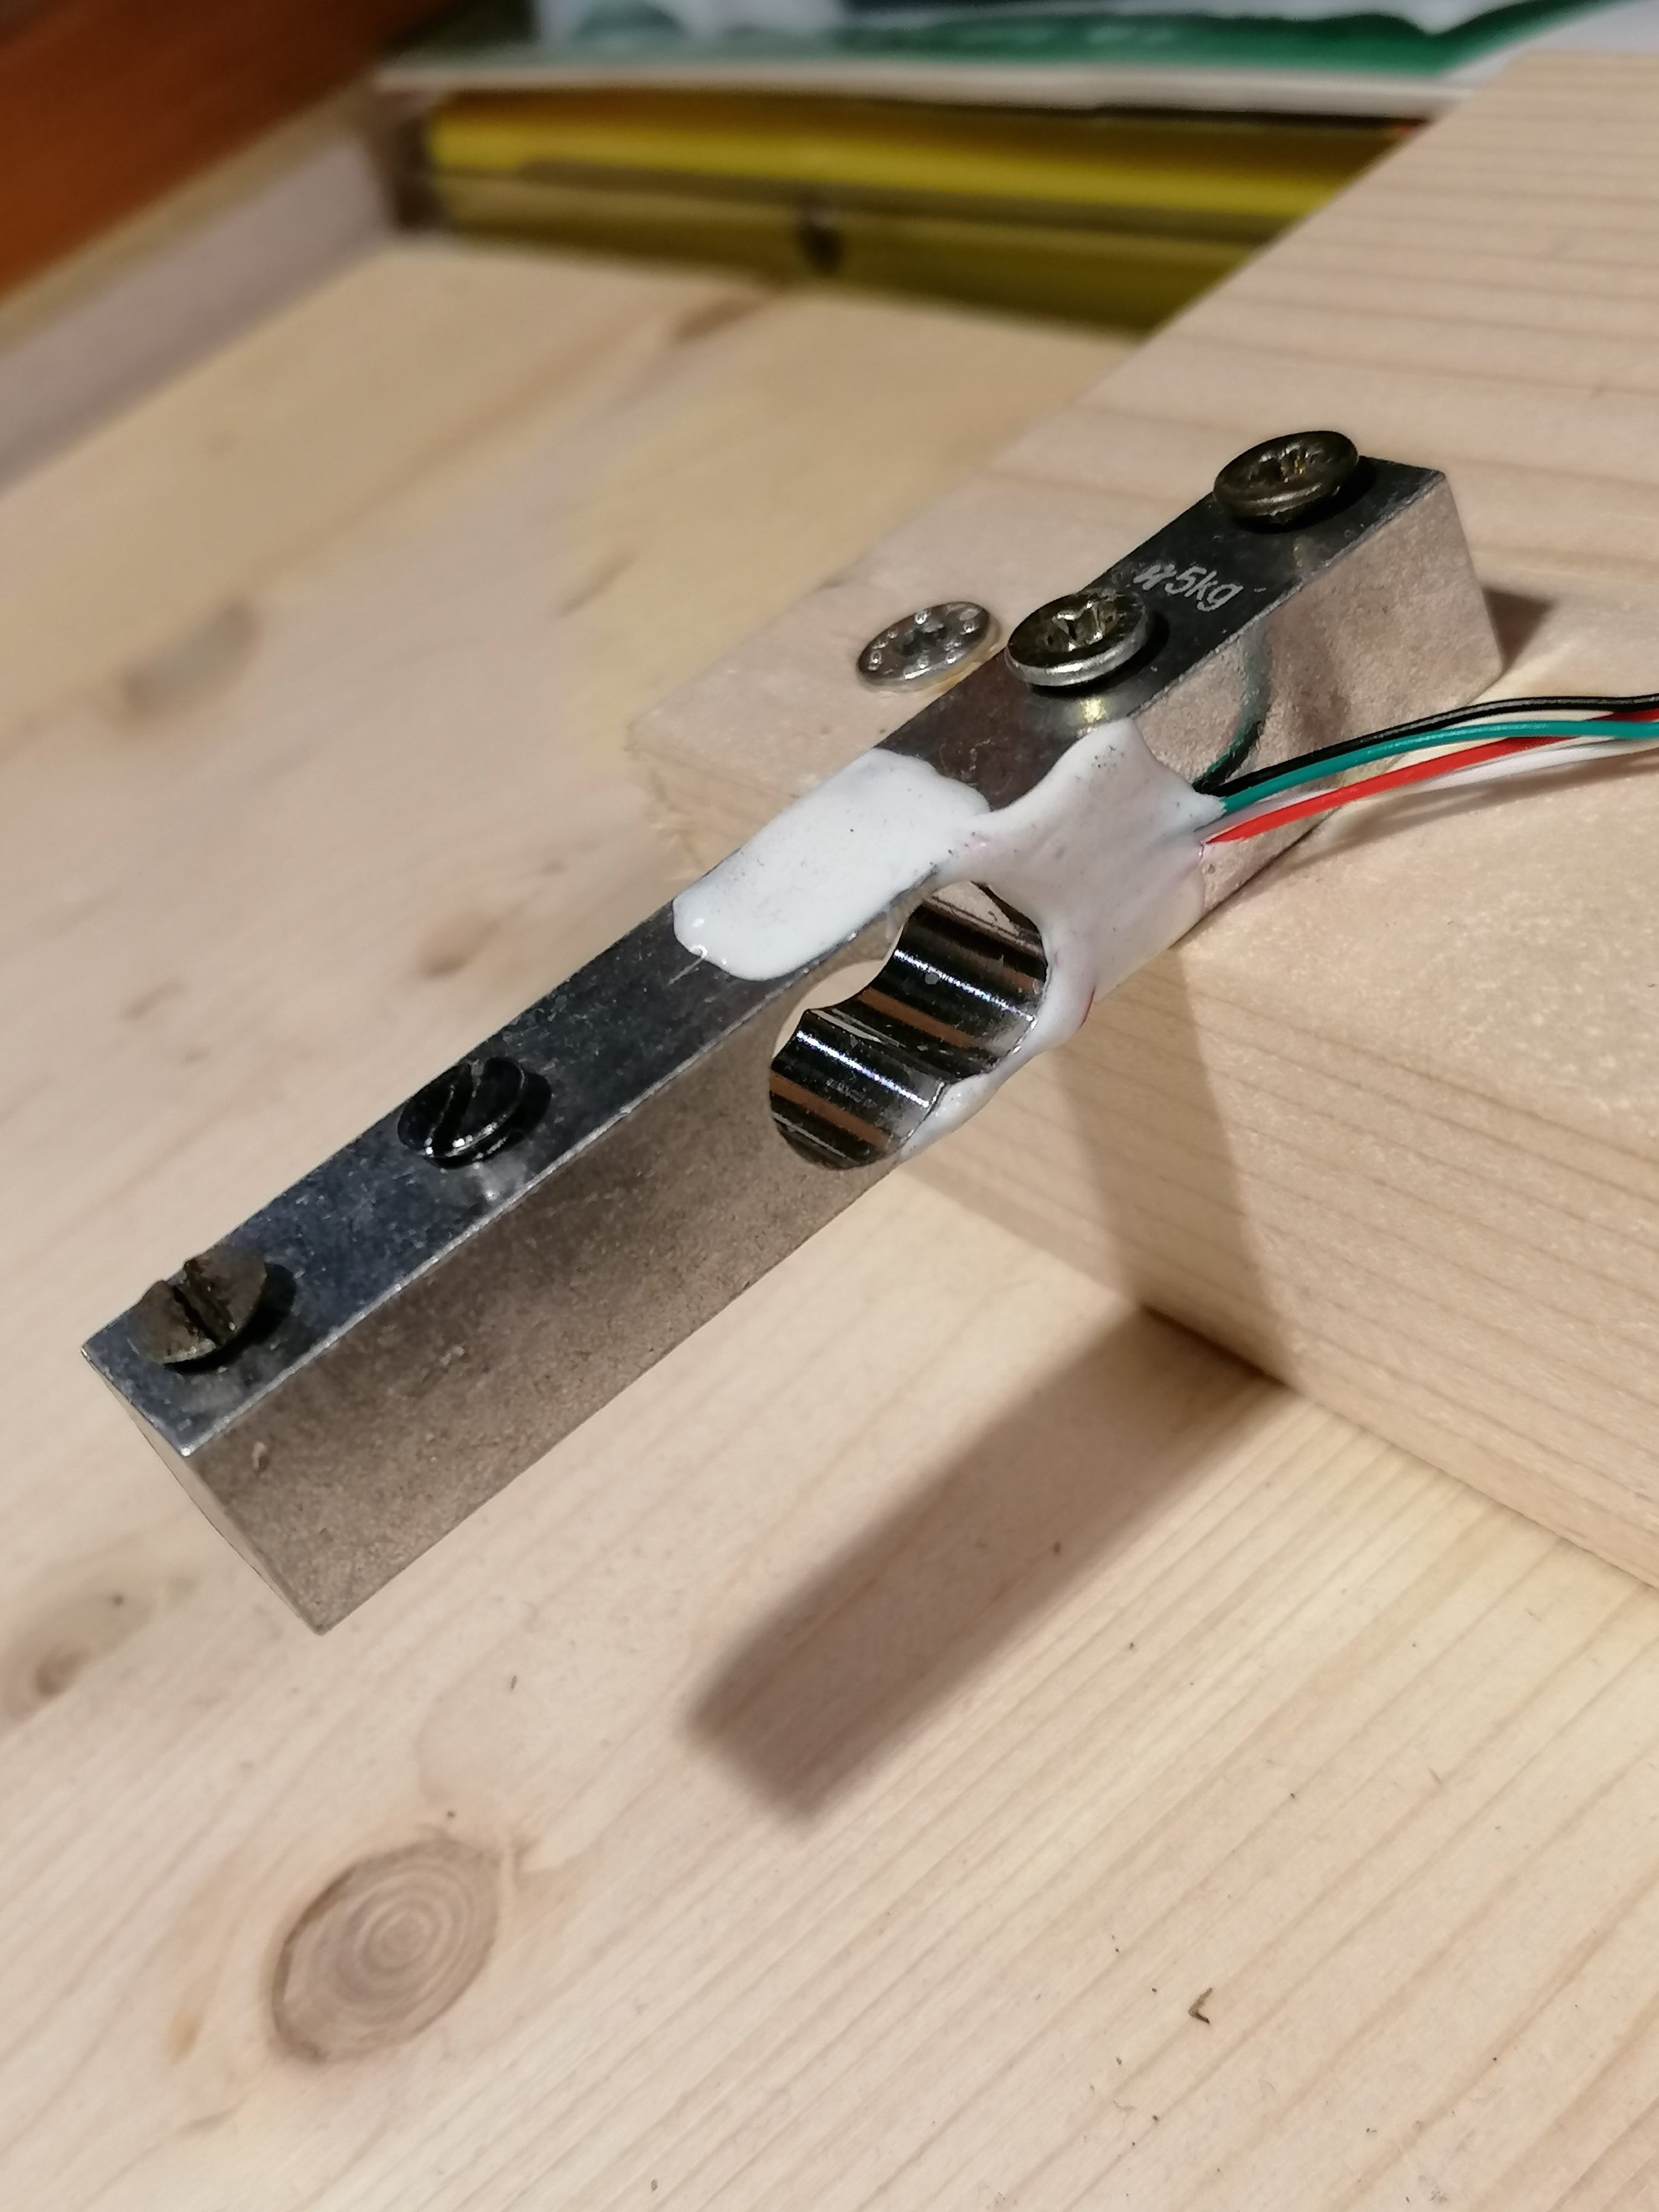
\includegraphics[width=0.3\textwidth]{waegezelle1.jpg}}
    \hfill
    \caption{Beide Versionen der Wägezellen}
\end{figure}

\subsection{IR-Sensor}

Zur Messung der Drehzahl wurde ein IR-Sensor gewählt, welcher über die gesamte Dauer des Projektes unverändert blieb.
Für erhöhte Genauigkeit bei den Messungen bot sich eine Ausführung mit höherer Messfrequenz an, da jedoch die anfängliche Variante befriedigende Ergebnisse lieferte wurde von dieser Änderung abgesehen.

Dieser Sensor liefert den Wert wie viel seines ausgestrahlten Lichts reflektiert wird, somit kann zwischen hellen und dunklen Oberflächen unterschieden werden.

Weitere Überlegungen hierzu finden sich unter \hyperref[drehzahlmessung]{\textit{Drehzahlmessung}} in Teil 5.

\begin{figure}[H]
    \begin{center}
        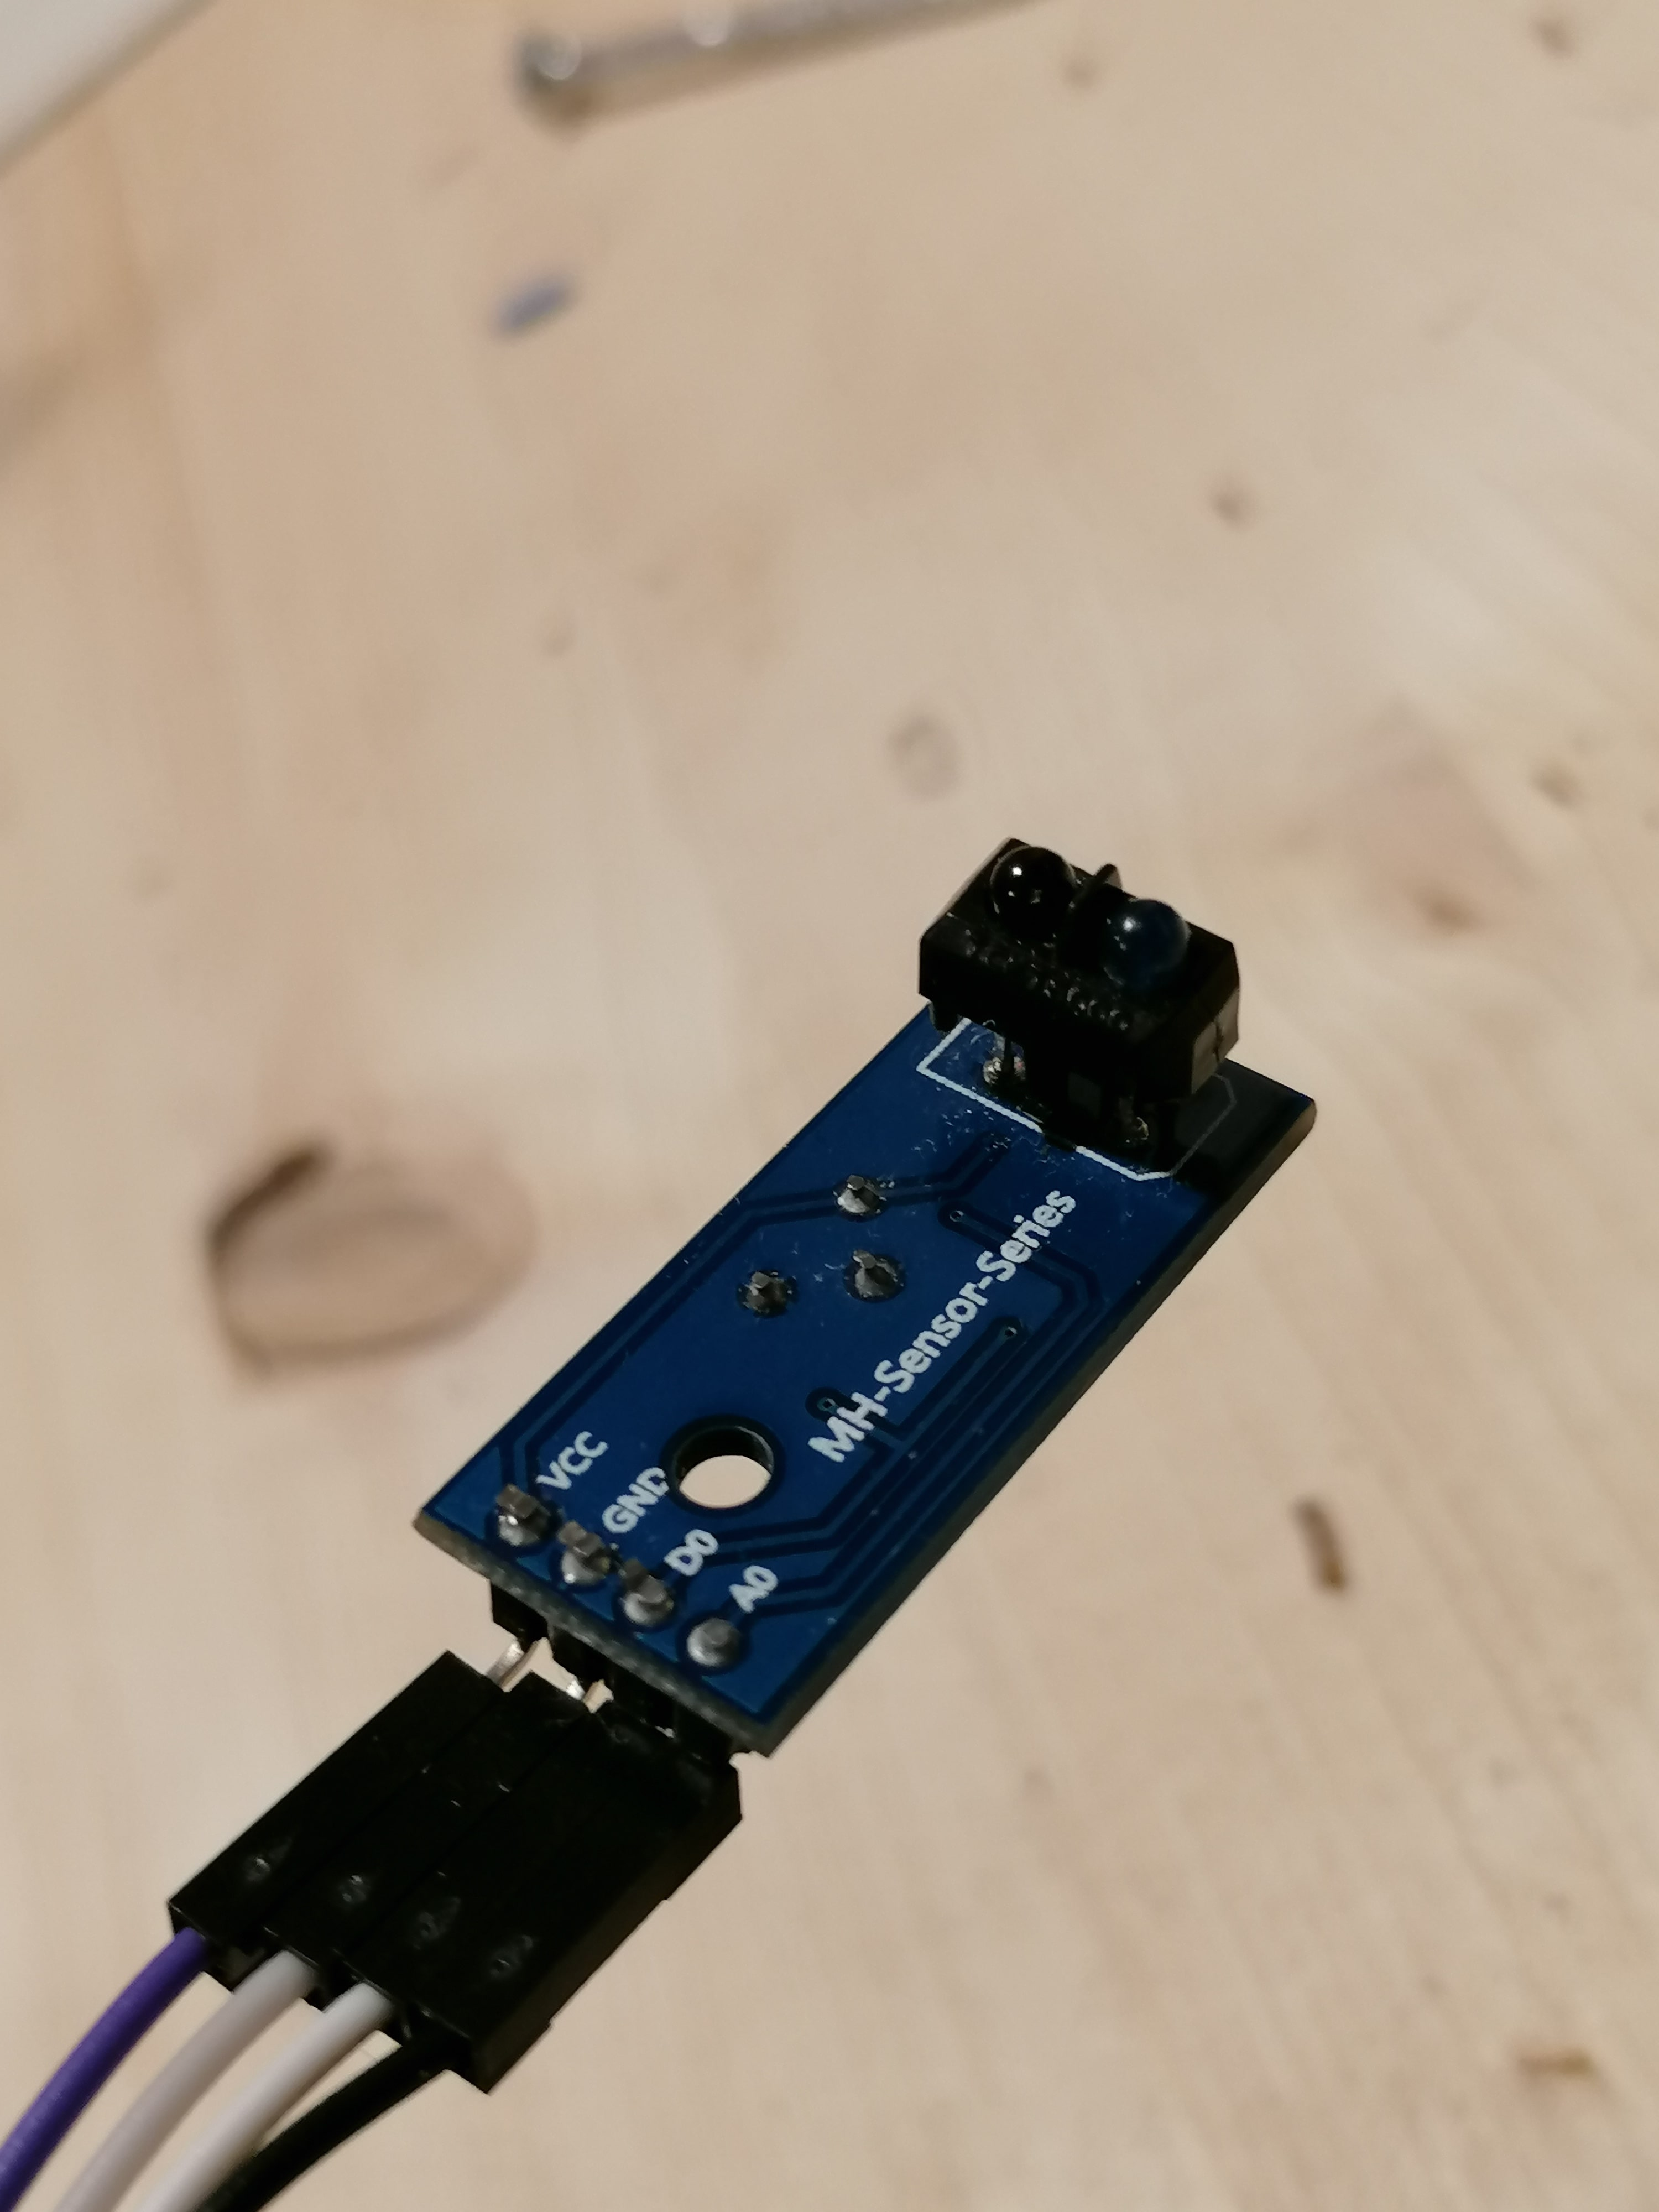
\includegraphics[width=0.3\textwidth]{irsensor.jpg}
        \caption{Der IR-Sensor}
    \end{center}
\end{figure}

\subsection{HX711}

Der HX711 wurde gewählt, da hier beinahe keine anderen Optionen zur Auswahl standen, sowie dieser das breiteste Angebot von Dokumentation zu dessen Verwendung besaß.

Da Veränderungen der Spannung durch die DMS nur minimal ist, muss diese zur Auswertung mit dem Arduino durch den HX711 Baustein verstärkt werden.

\begin{figure}[H]
    \begin{center}
        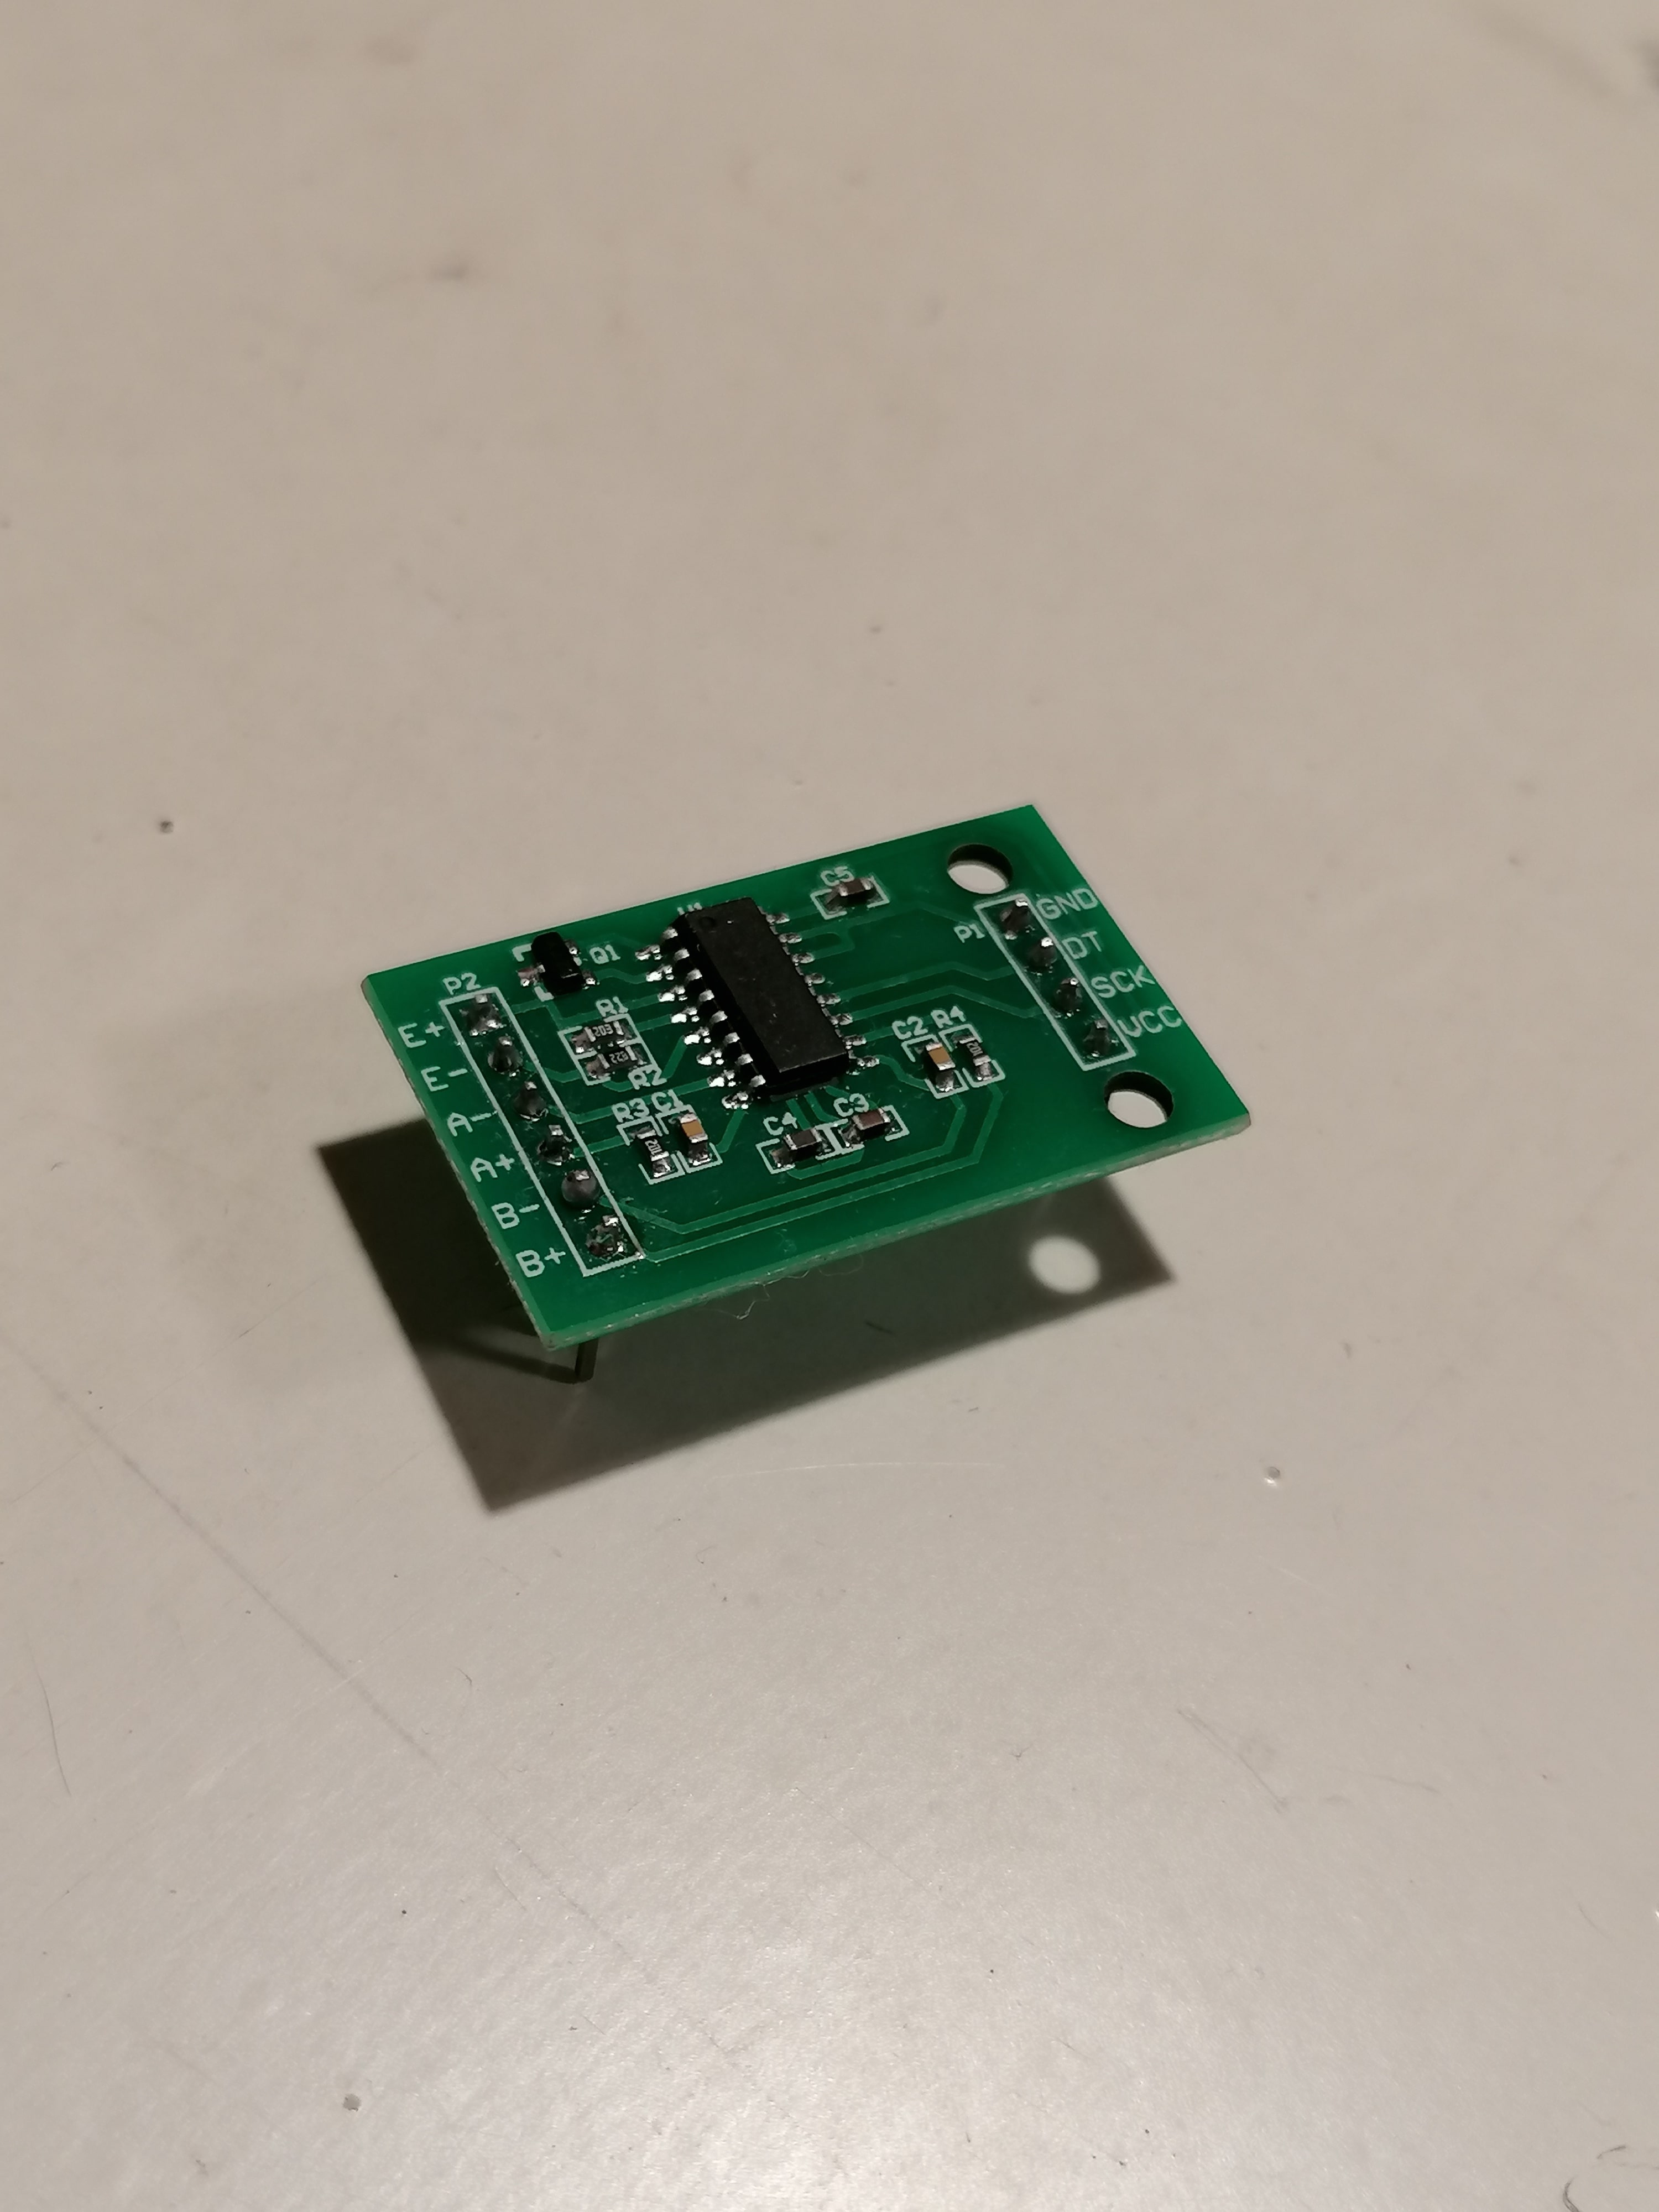
\includegraphics[width=0.3\textwidth]{hx711.jpg}
        \caption{Der HX711 Verstärkerbaustein}
    \end{center}
\end{figure}

\subsection{Arduino Nano}

Auch hier war die zu treffende Entscheidung sehr einfach.
Trotz der Menge an Alternativen beinflusste hier der Faktor, dass die Verwendung des Arduino Nano aufgrund der Verwendung im Unterricht bereits gängig war diese Entscheidung am meisten.

\begin{figure}[H]
    \centering
    \hfill
    \subfigure[Arduino Nano]{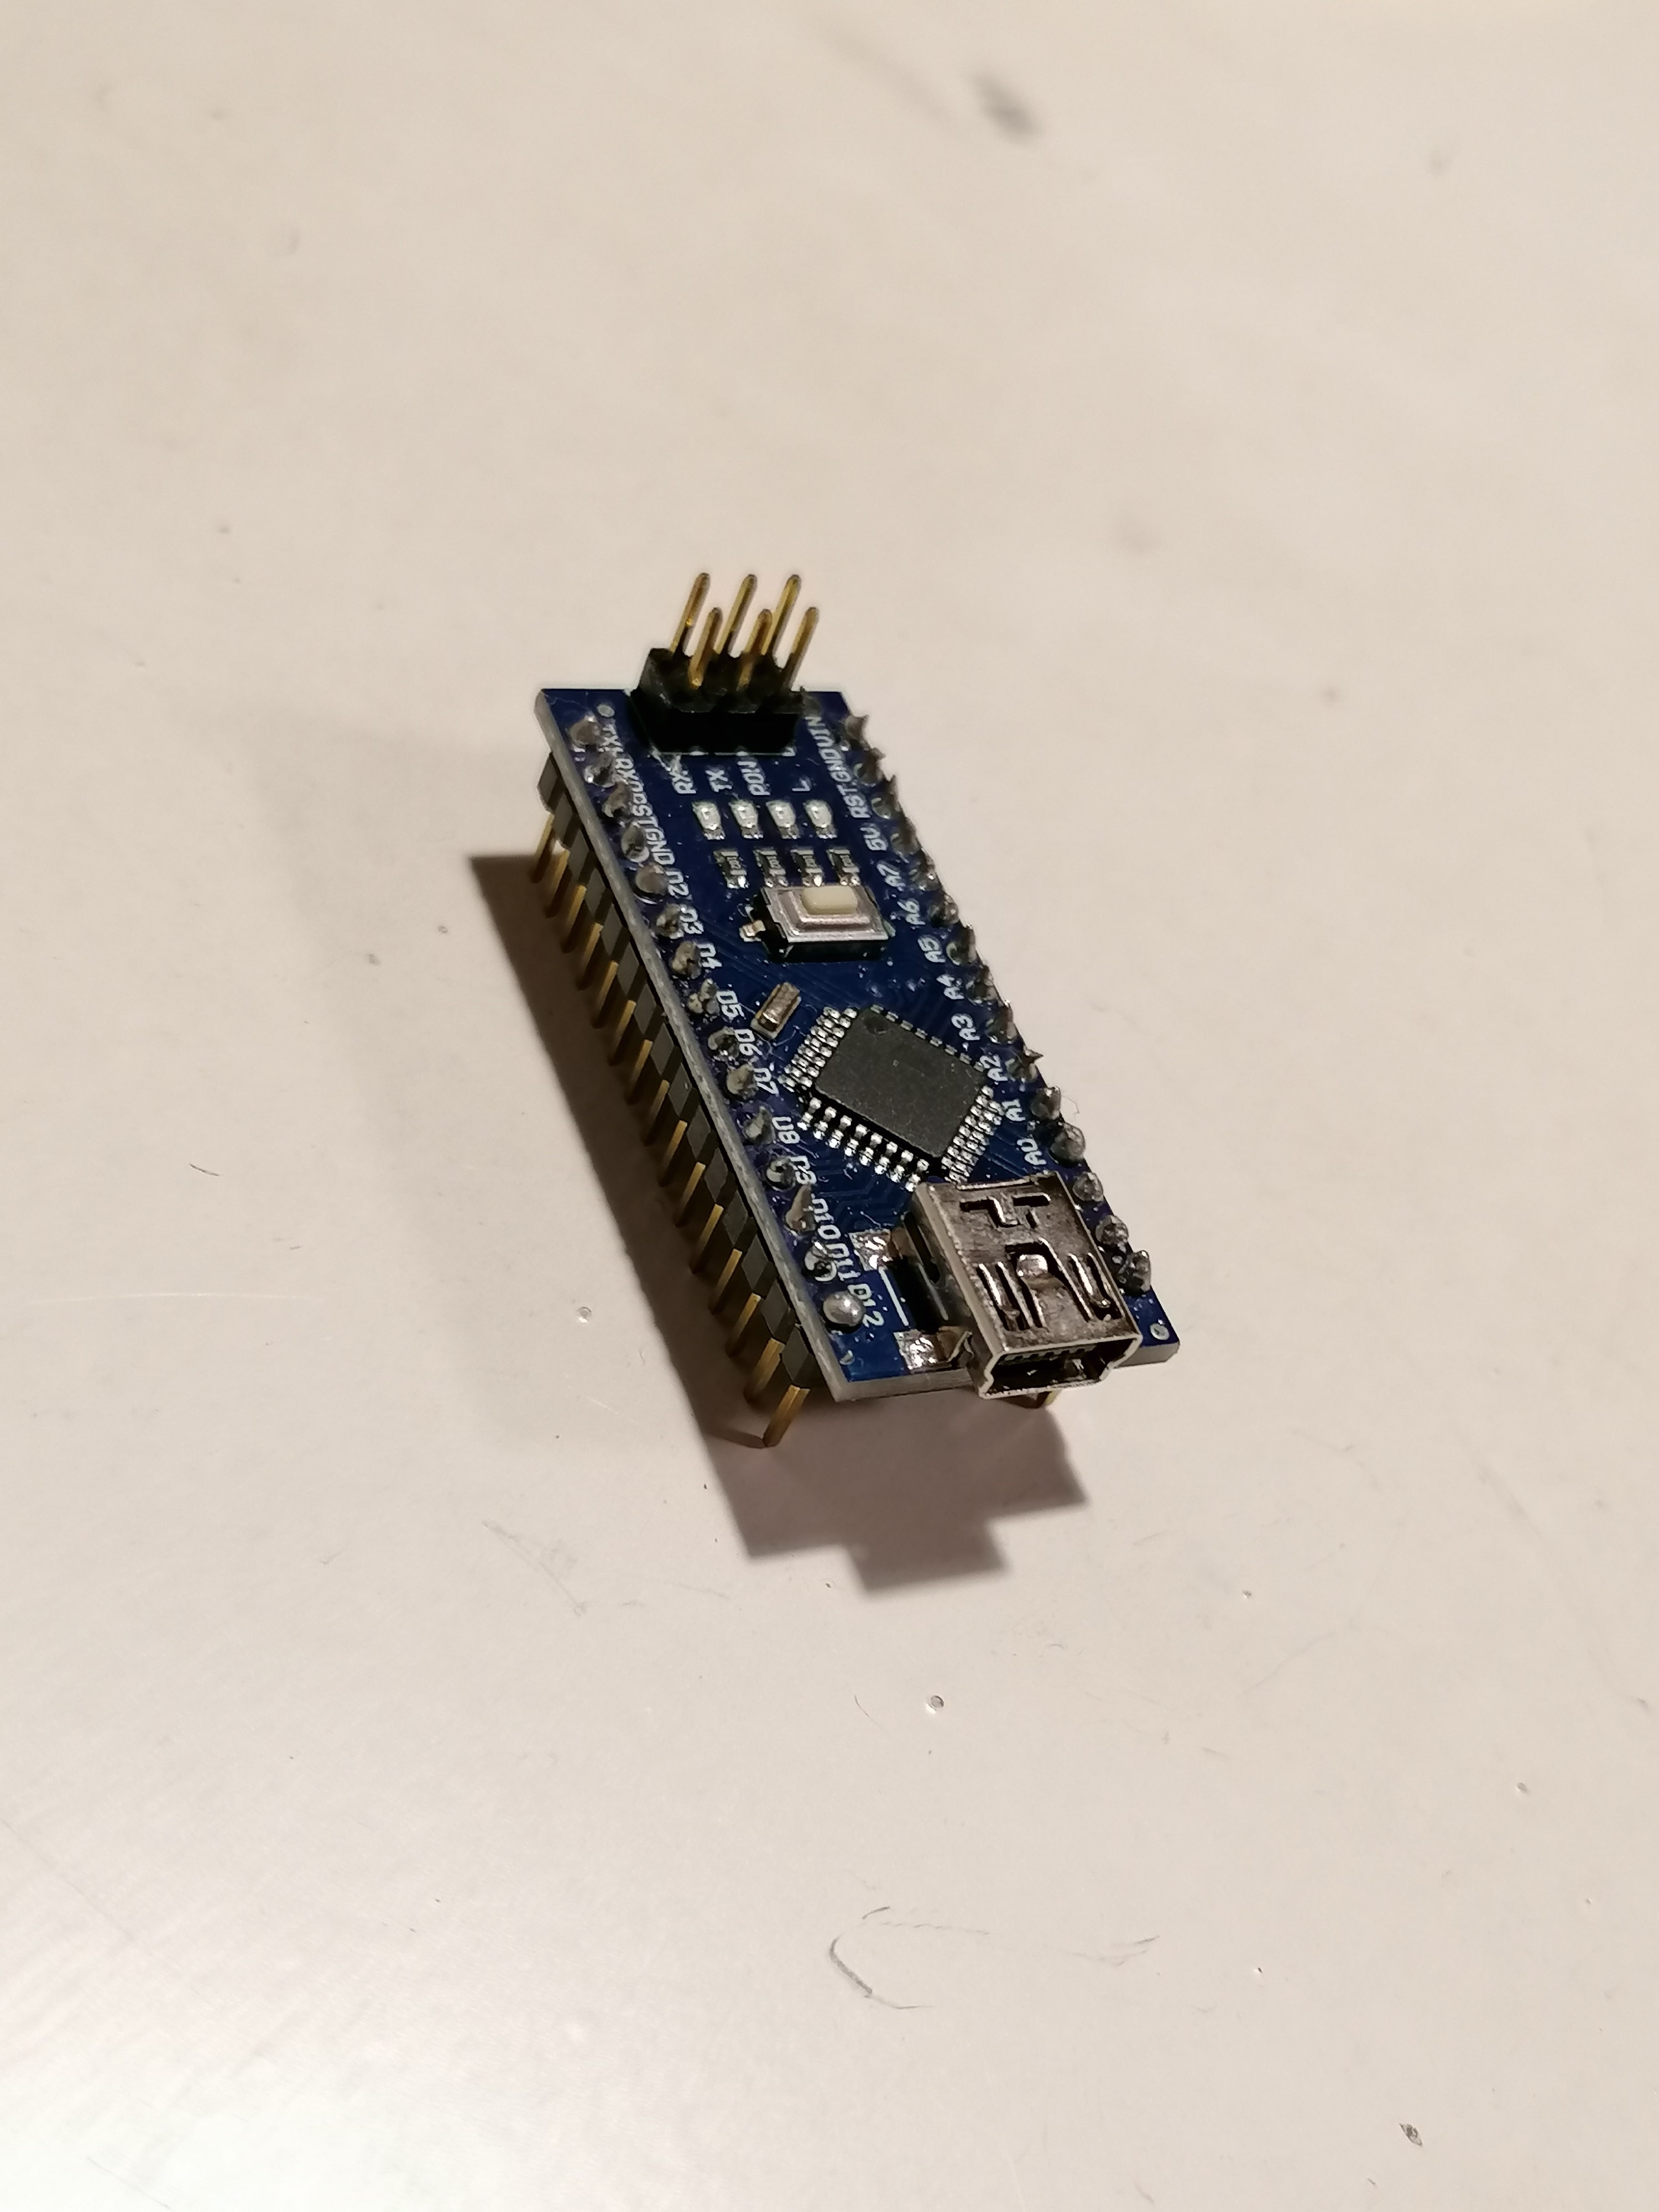
\includegraphics[width=0.3\textwidth]{arduino.jpg}}
    \hfill
    \subfigure[Arduino Kit]{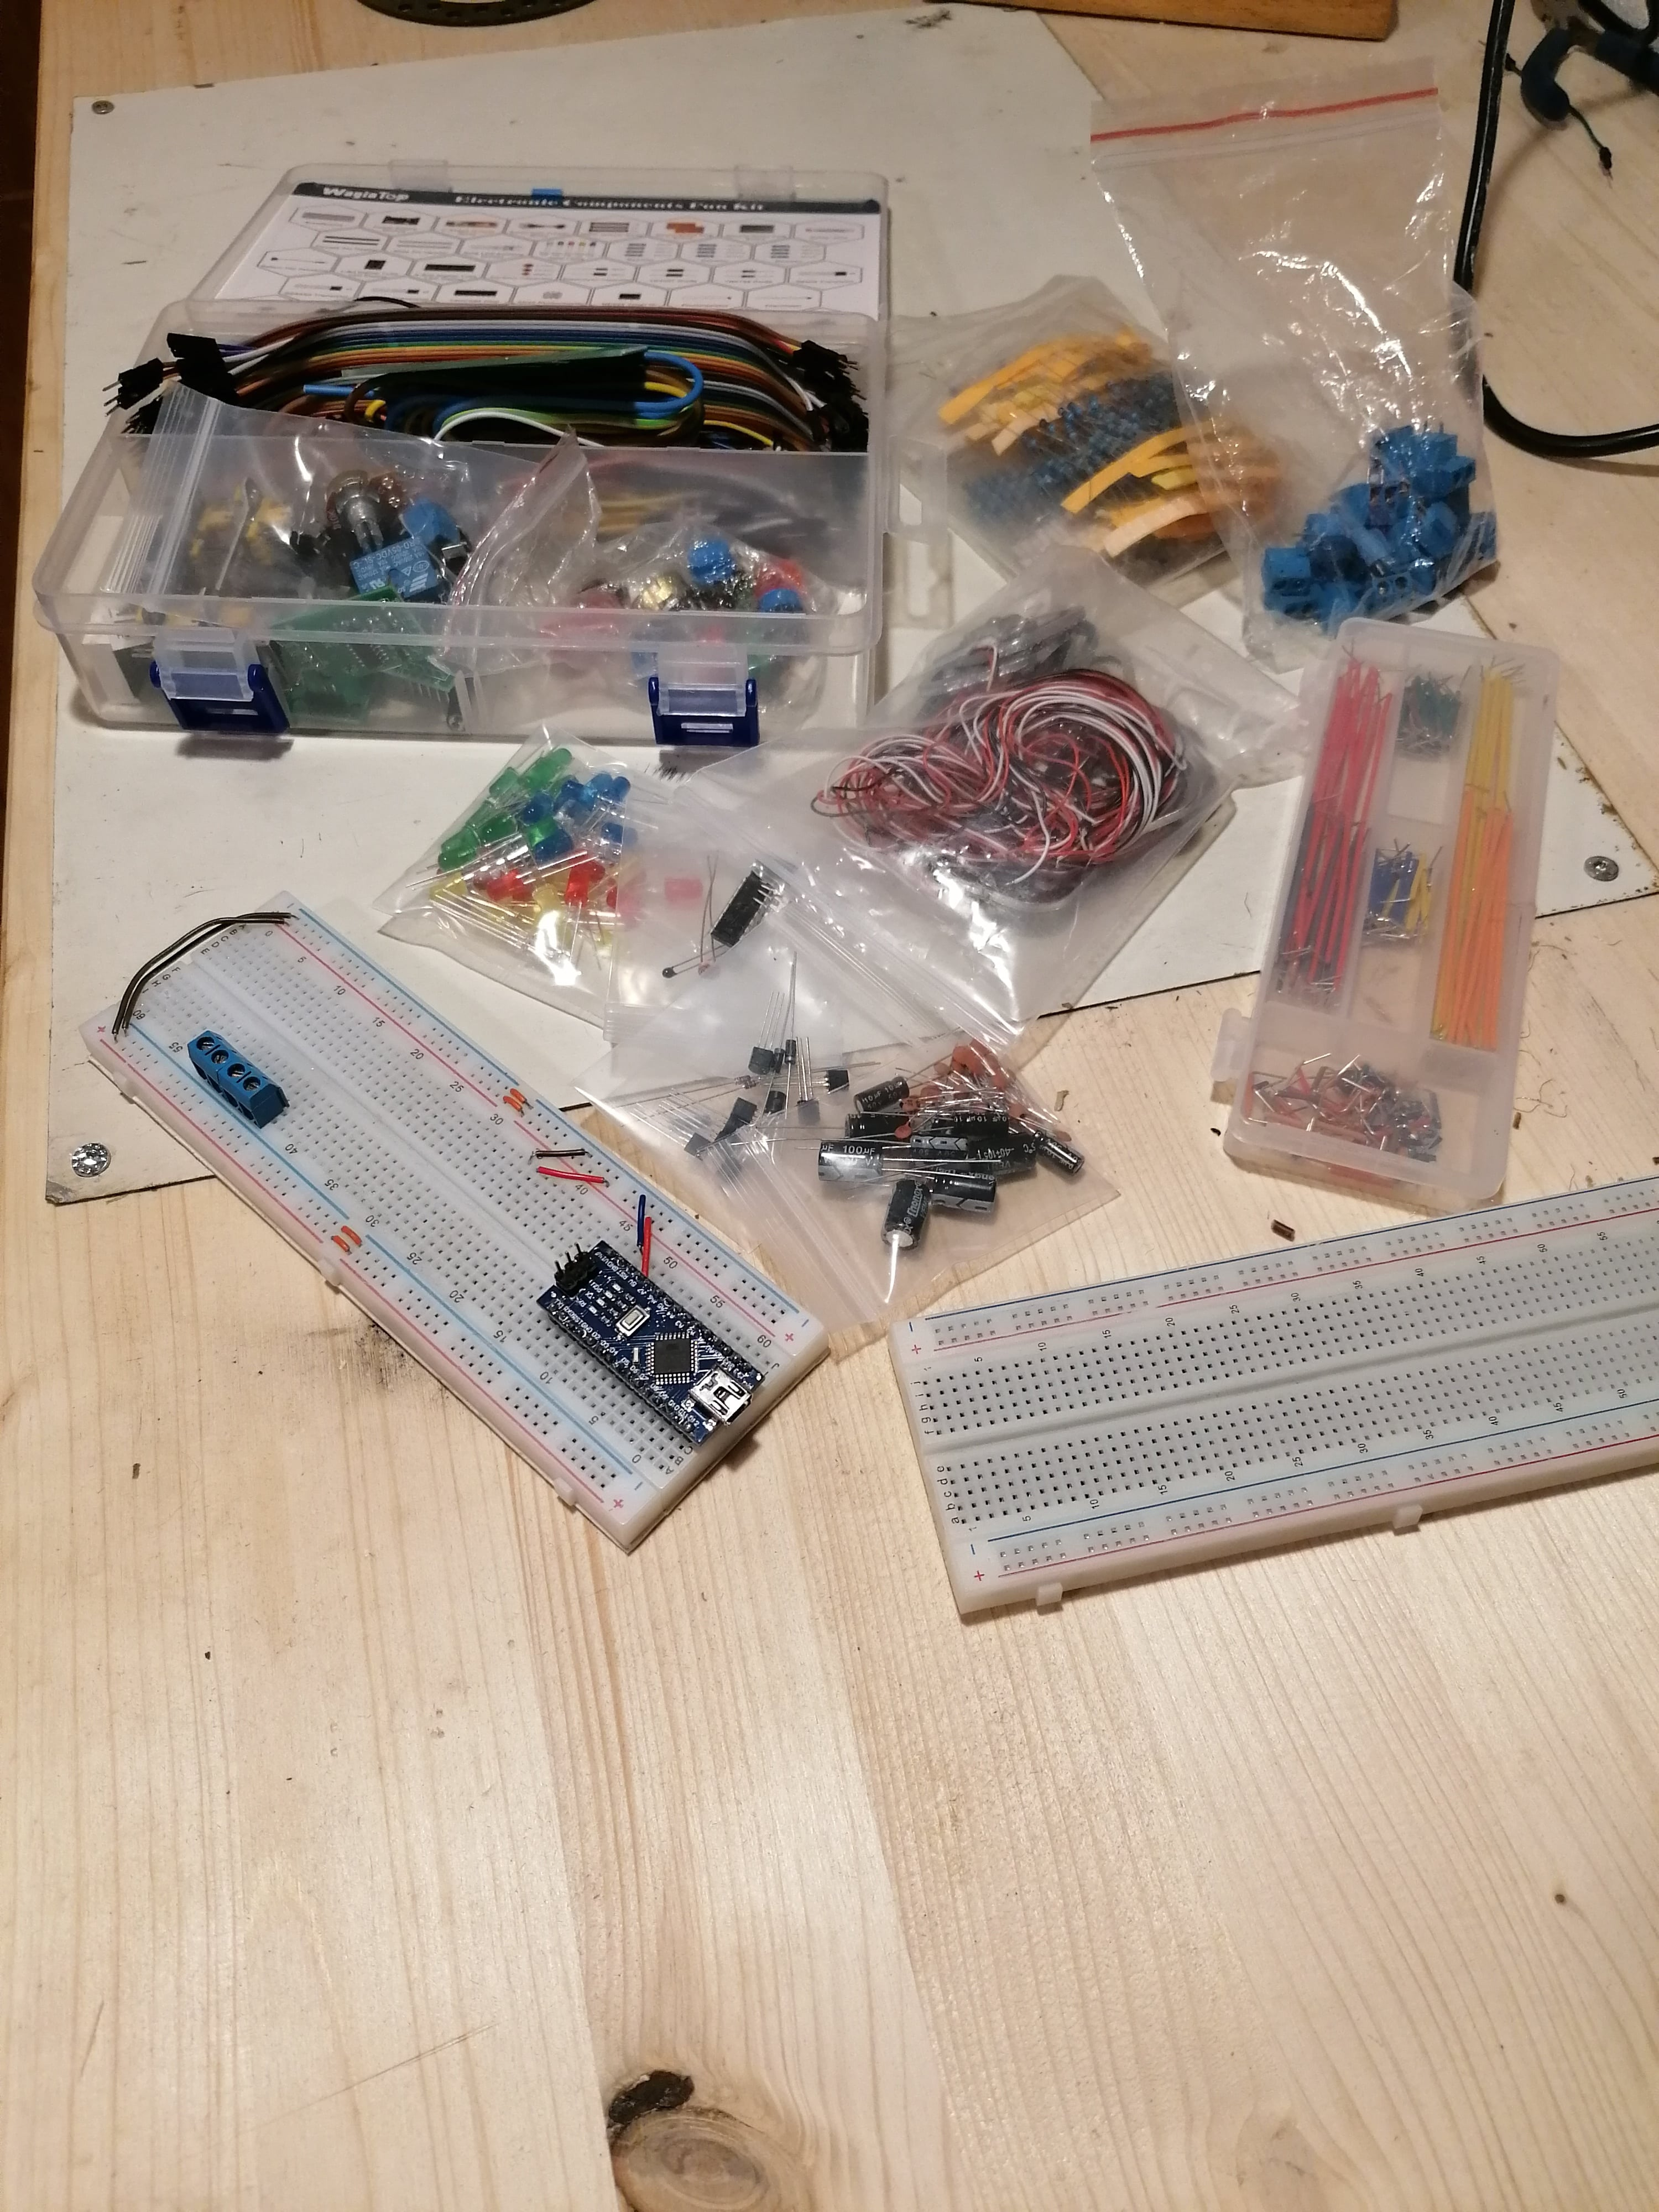
\includegraphics[width=0.3\textwidth]{arduinokit.jpg}}
    \hfill
    \caption{Arduino und Arduino Kit für die Versuche}
\end{figure}

\subsection{Rohrschelle}

Zur Montage des Armes, über welchen das Drehmoment abgelesen wird, wurde eine Rohrschelle gewählt.
Dies bot sich aufgrund der geringen Kosten, sowie der simplen Verwendung an.

Auch hier finden sich weitere Überlegungen in Teil 5 unter dem Punkt \hyperref[rohrschelle]{\textit{Rohrschelle}}.

\begin{figure}[H]
    \begin{center}
        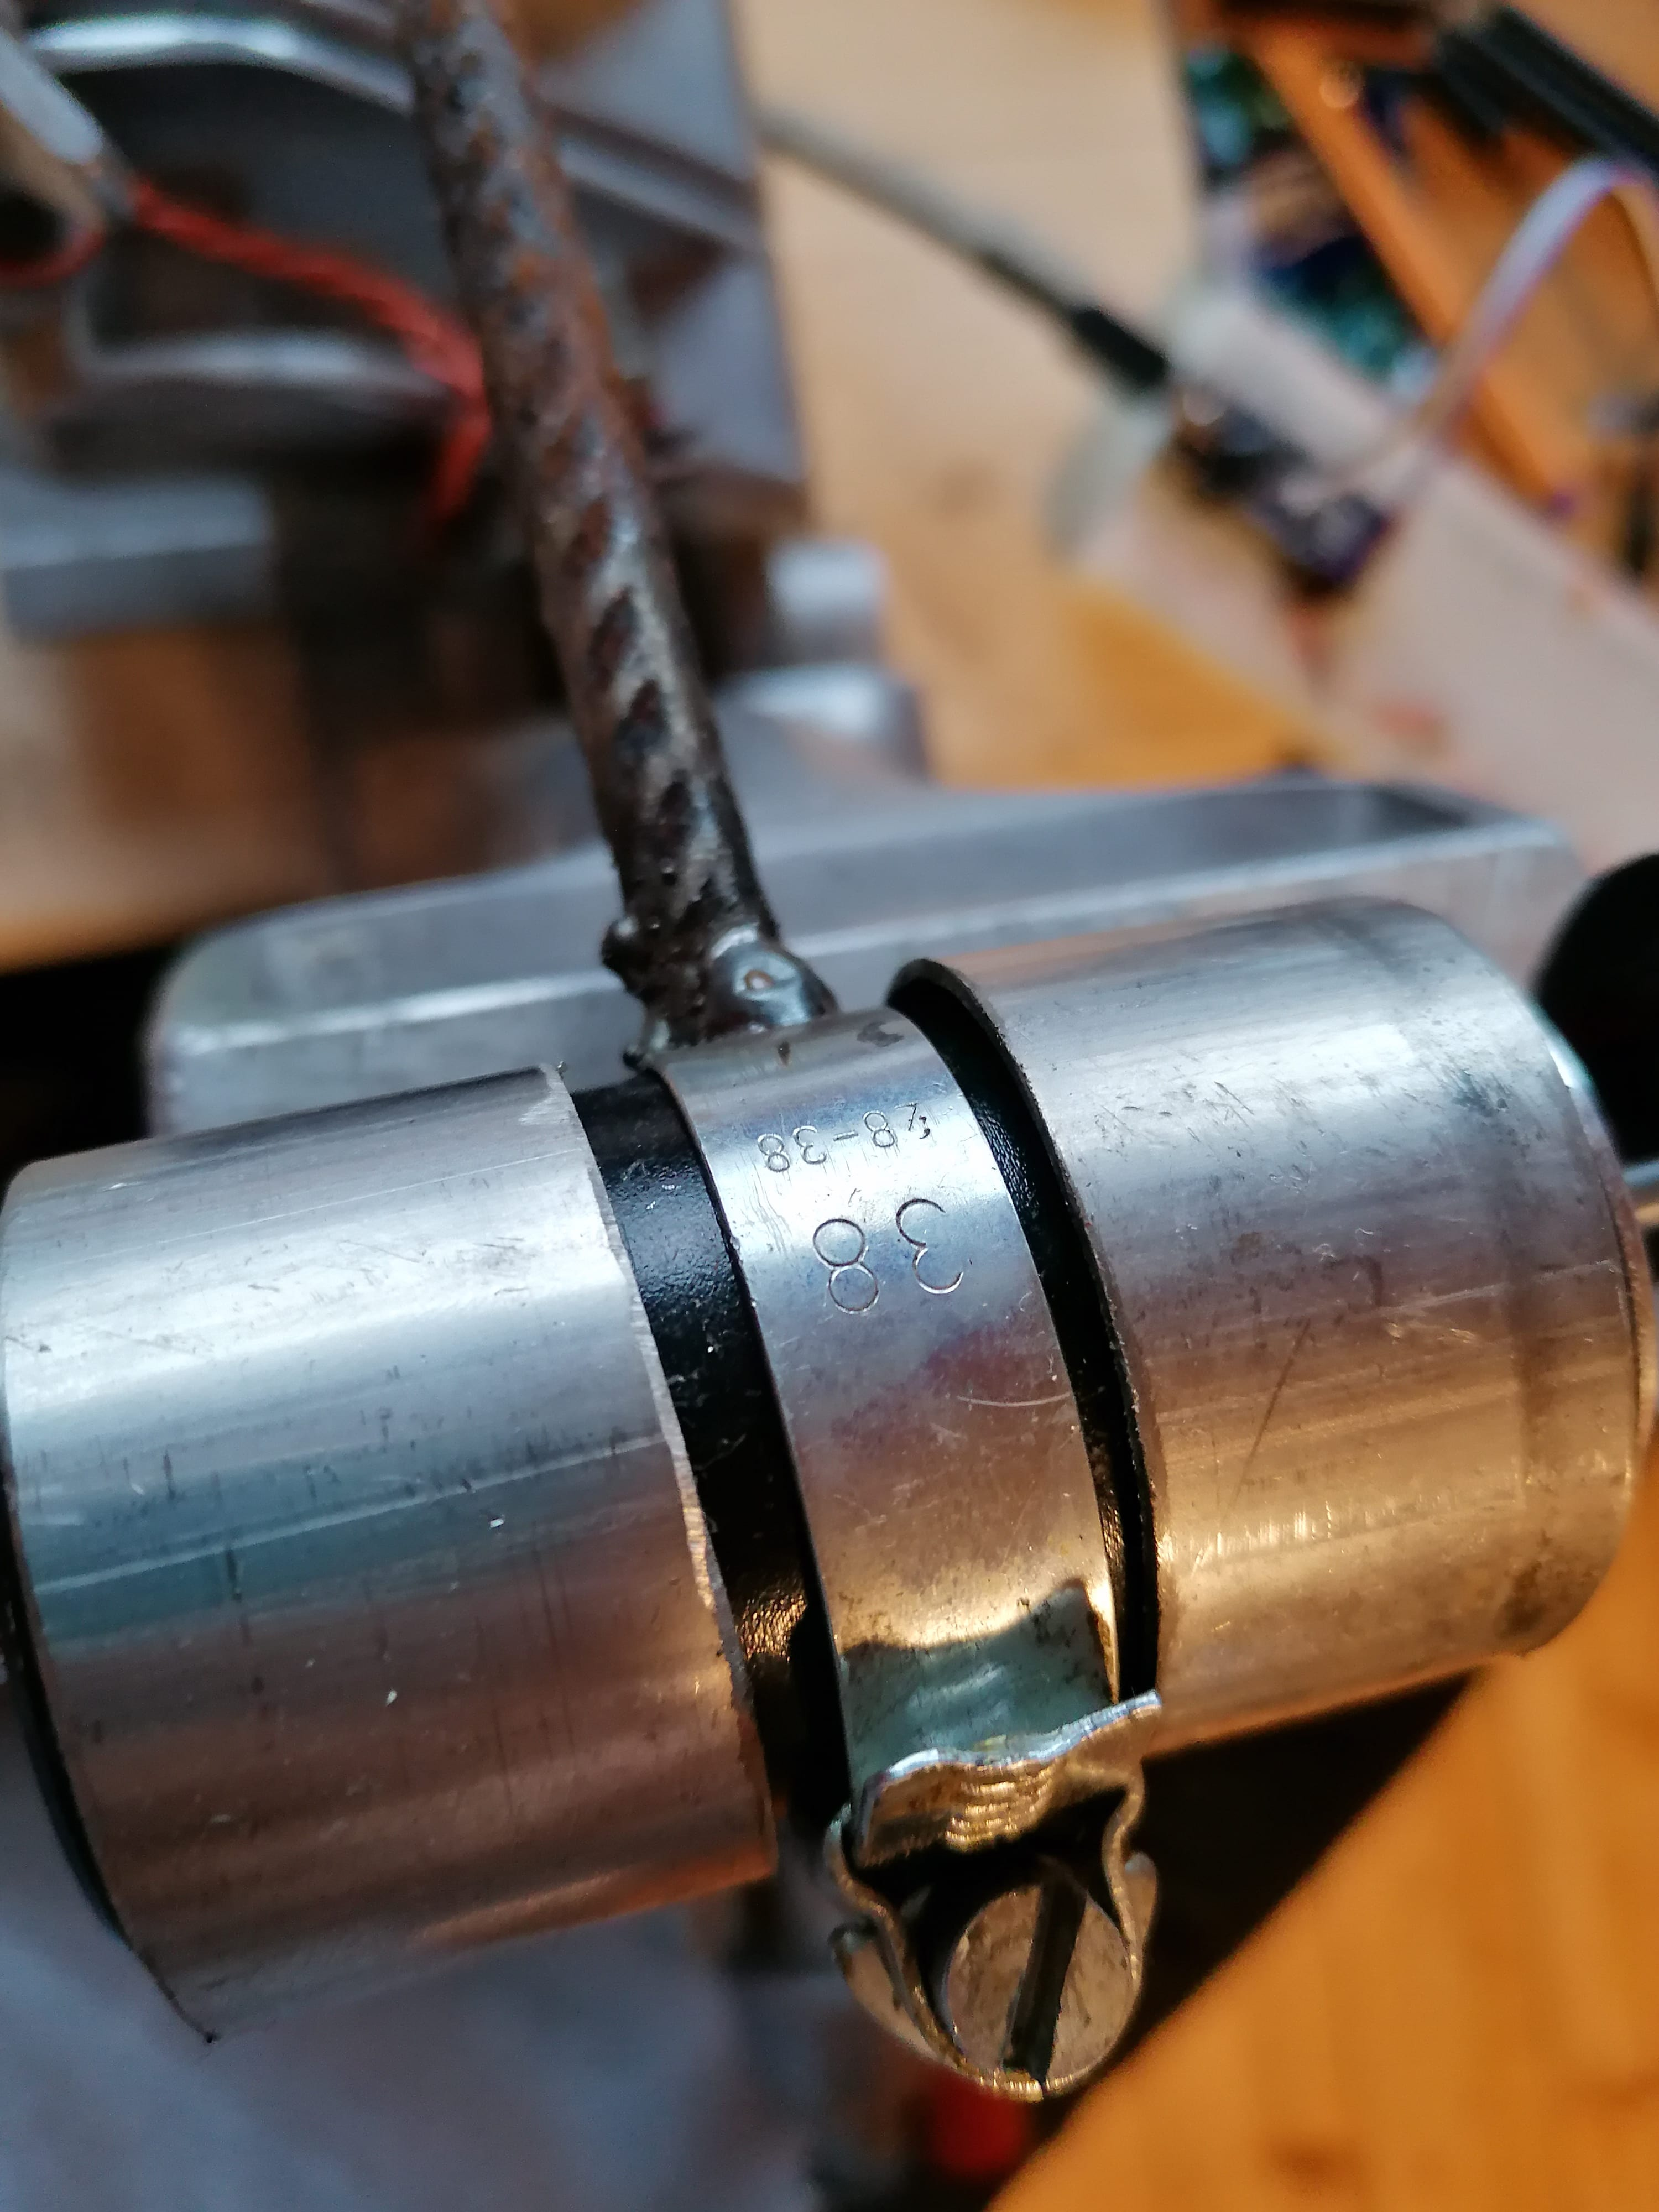
\includegraphics[width=0.3\textwidth]{rohrschelle.jpg}
        \caption{Die Rohrschelle mit angeschweißtem Arm}
    \end{center}
\end{figure}

\subsection{Bremse}

Zum Bremsen wurde eine Bremsscheibe mit einem mechanischen Bremsschuh gewählt.
Hier wurde die kleinste Ausführung gewählt, um die Größe des Versuchsaufbaues gering zu halten.

Alternativen finden sich in Teil 5 unter \hyperref[gegenkupplung]{\textit{Gegenkupplung}}.

\begin{figure}[H]
    \centering
    \hfill
    \subfigure[Bremsscheibe 120mm]{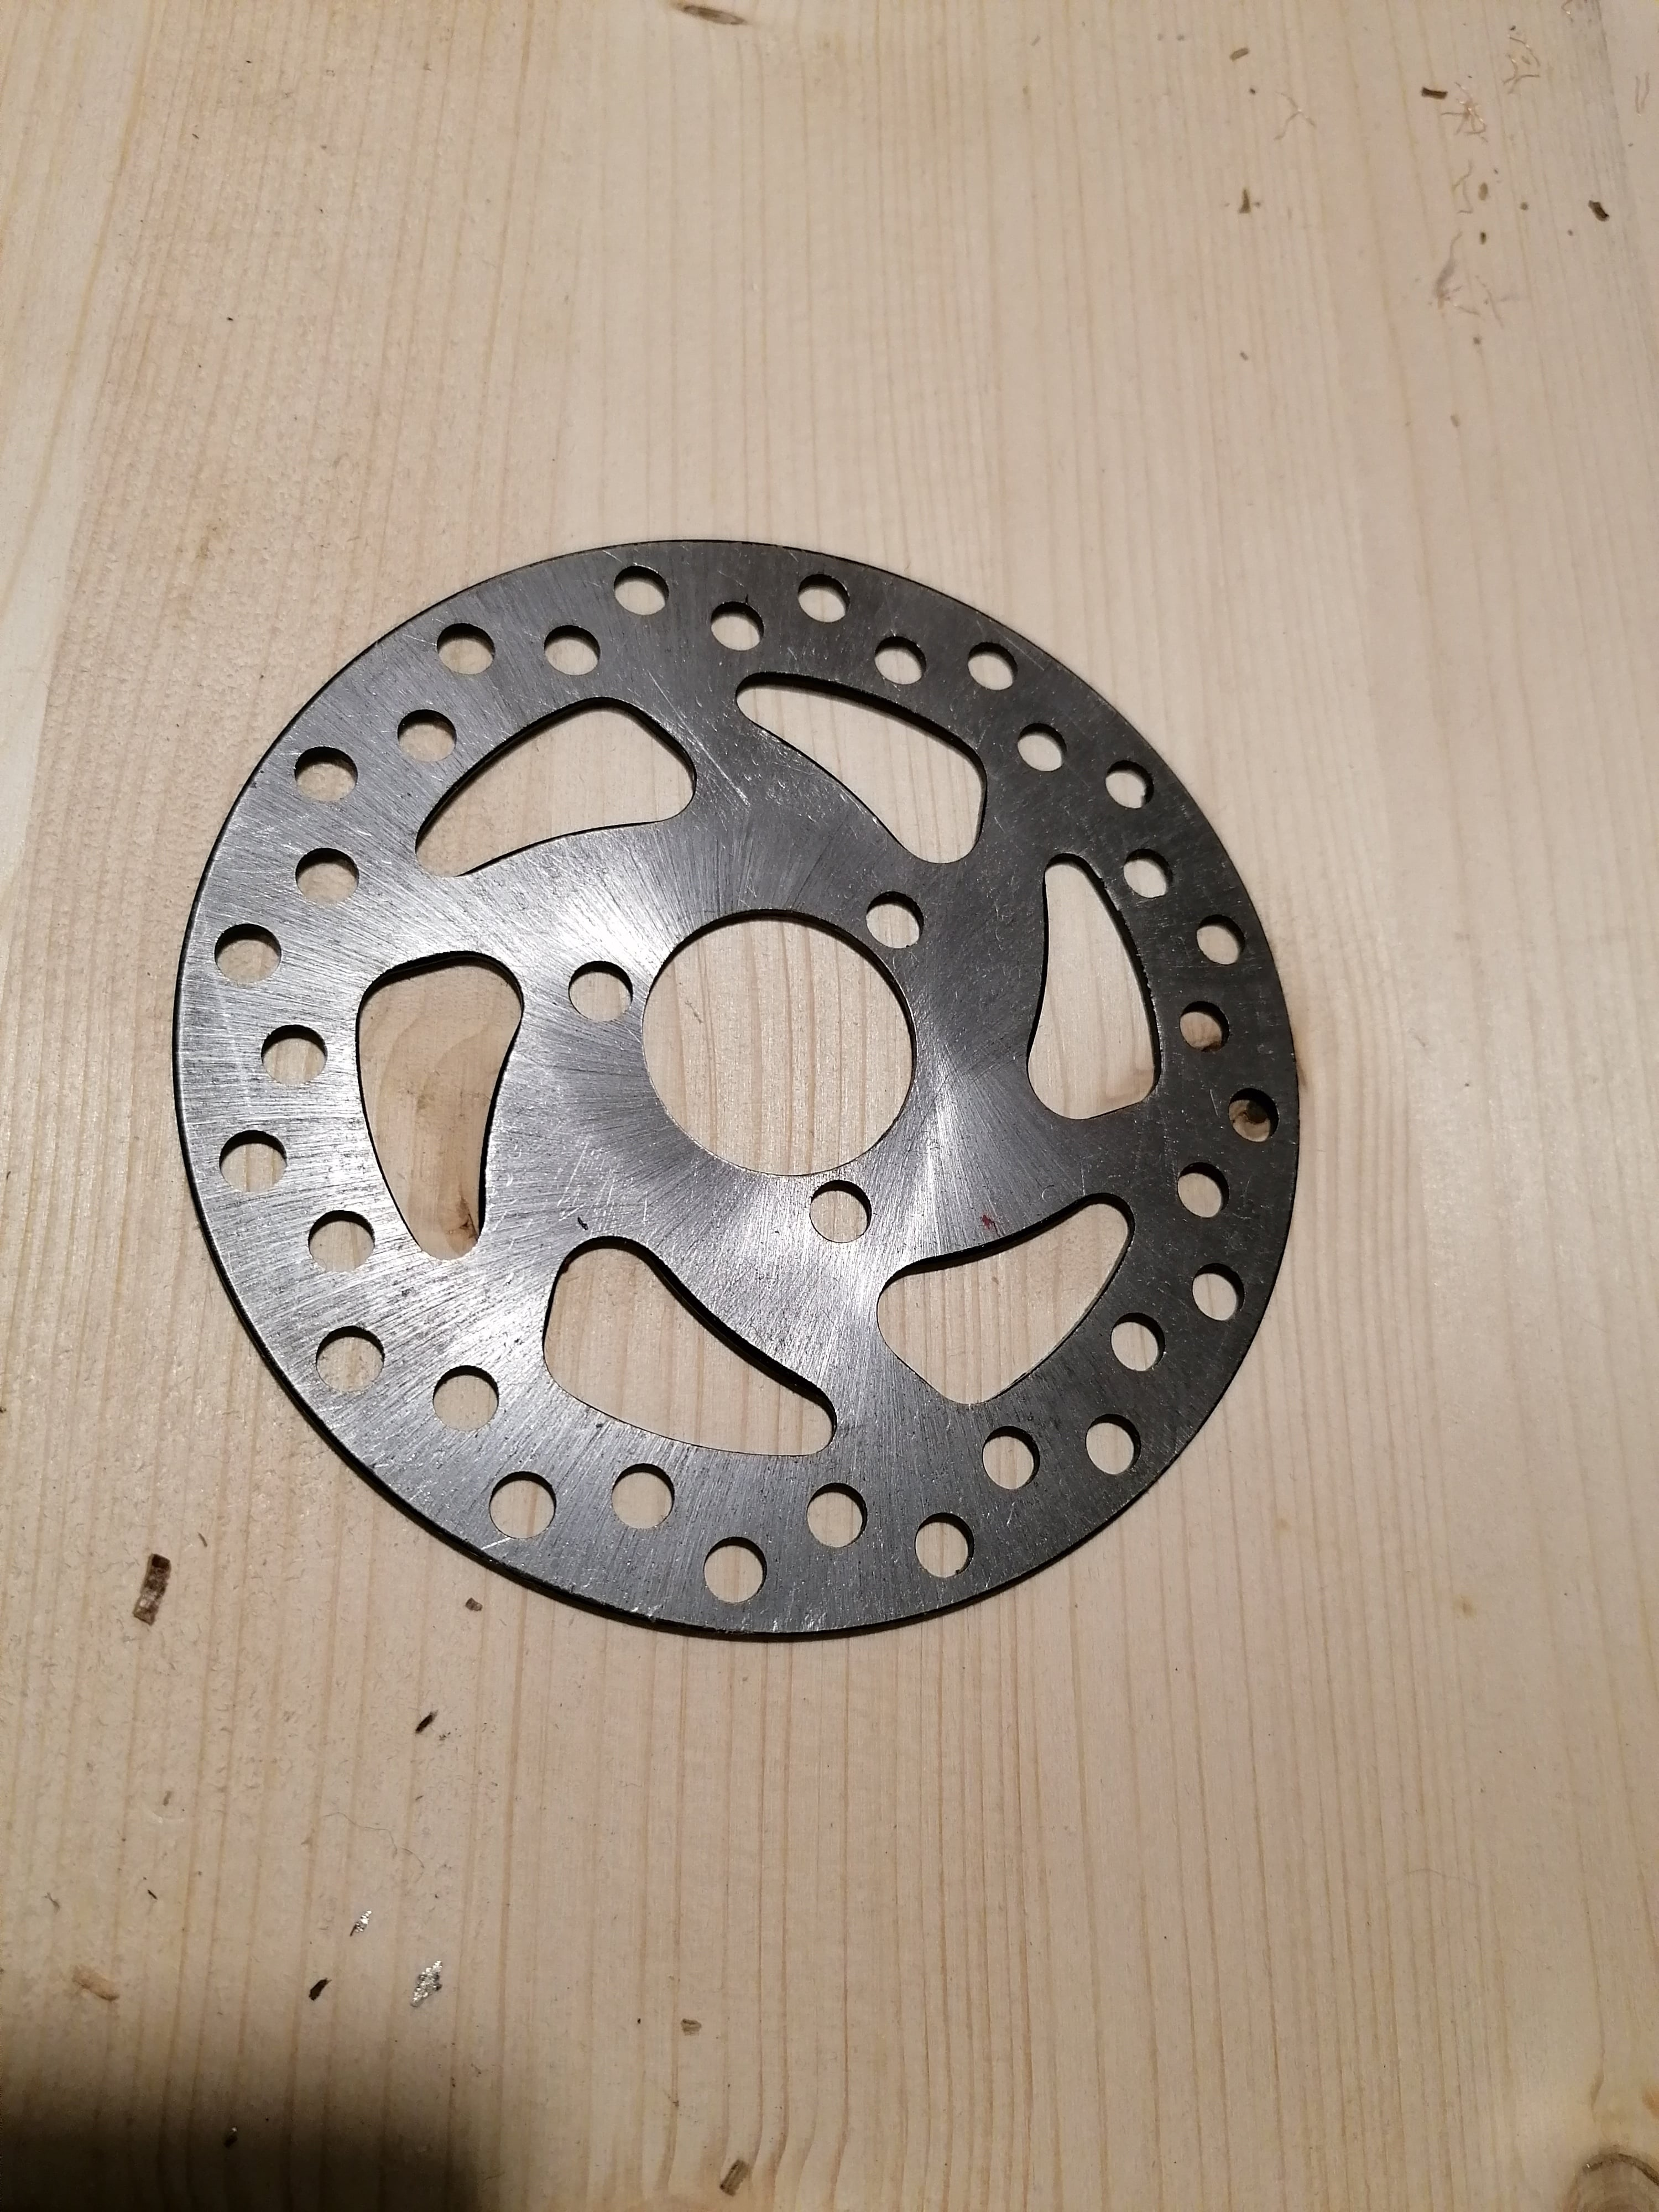
\includegraphics[width=0.3\textwidth]{bremsscheibe.jpg}}
    \hfill
    \subfigure[Bremssattel zu Bremsscheibe]{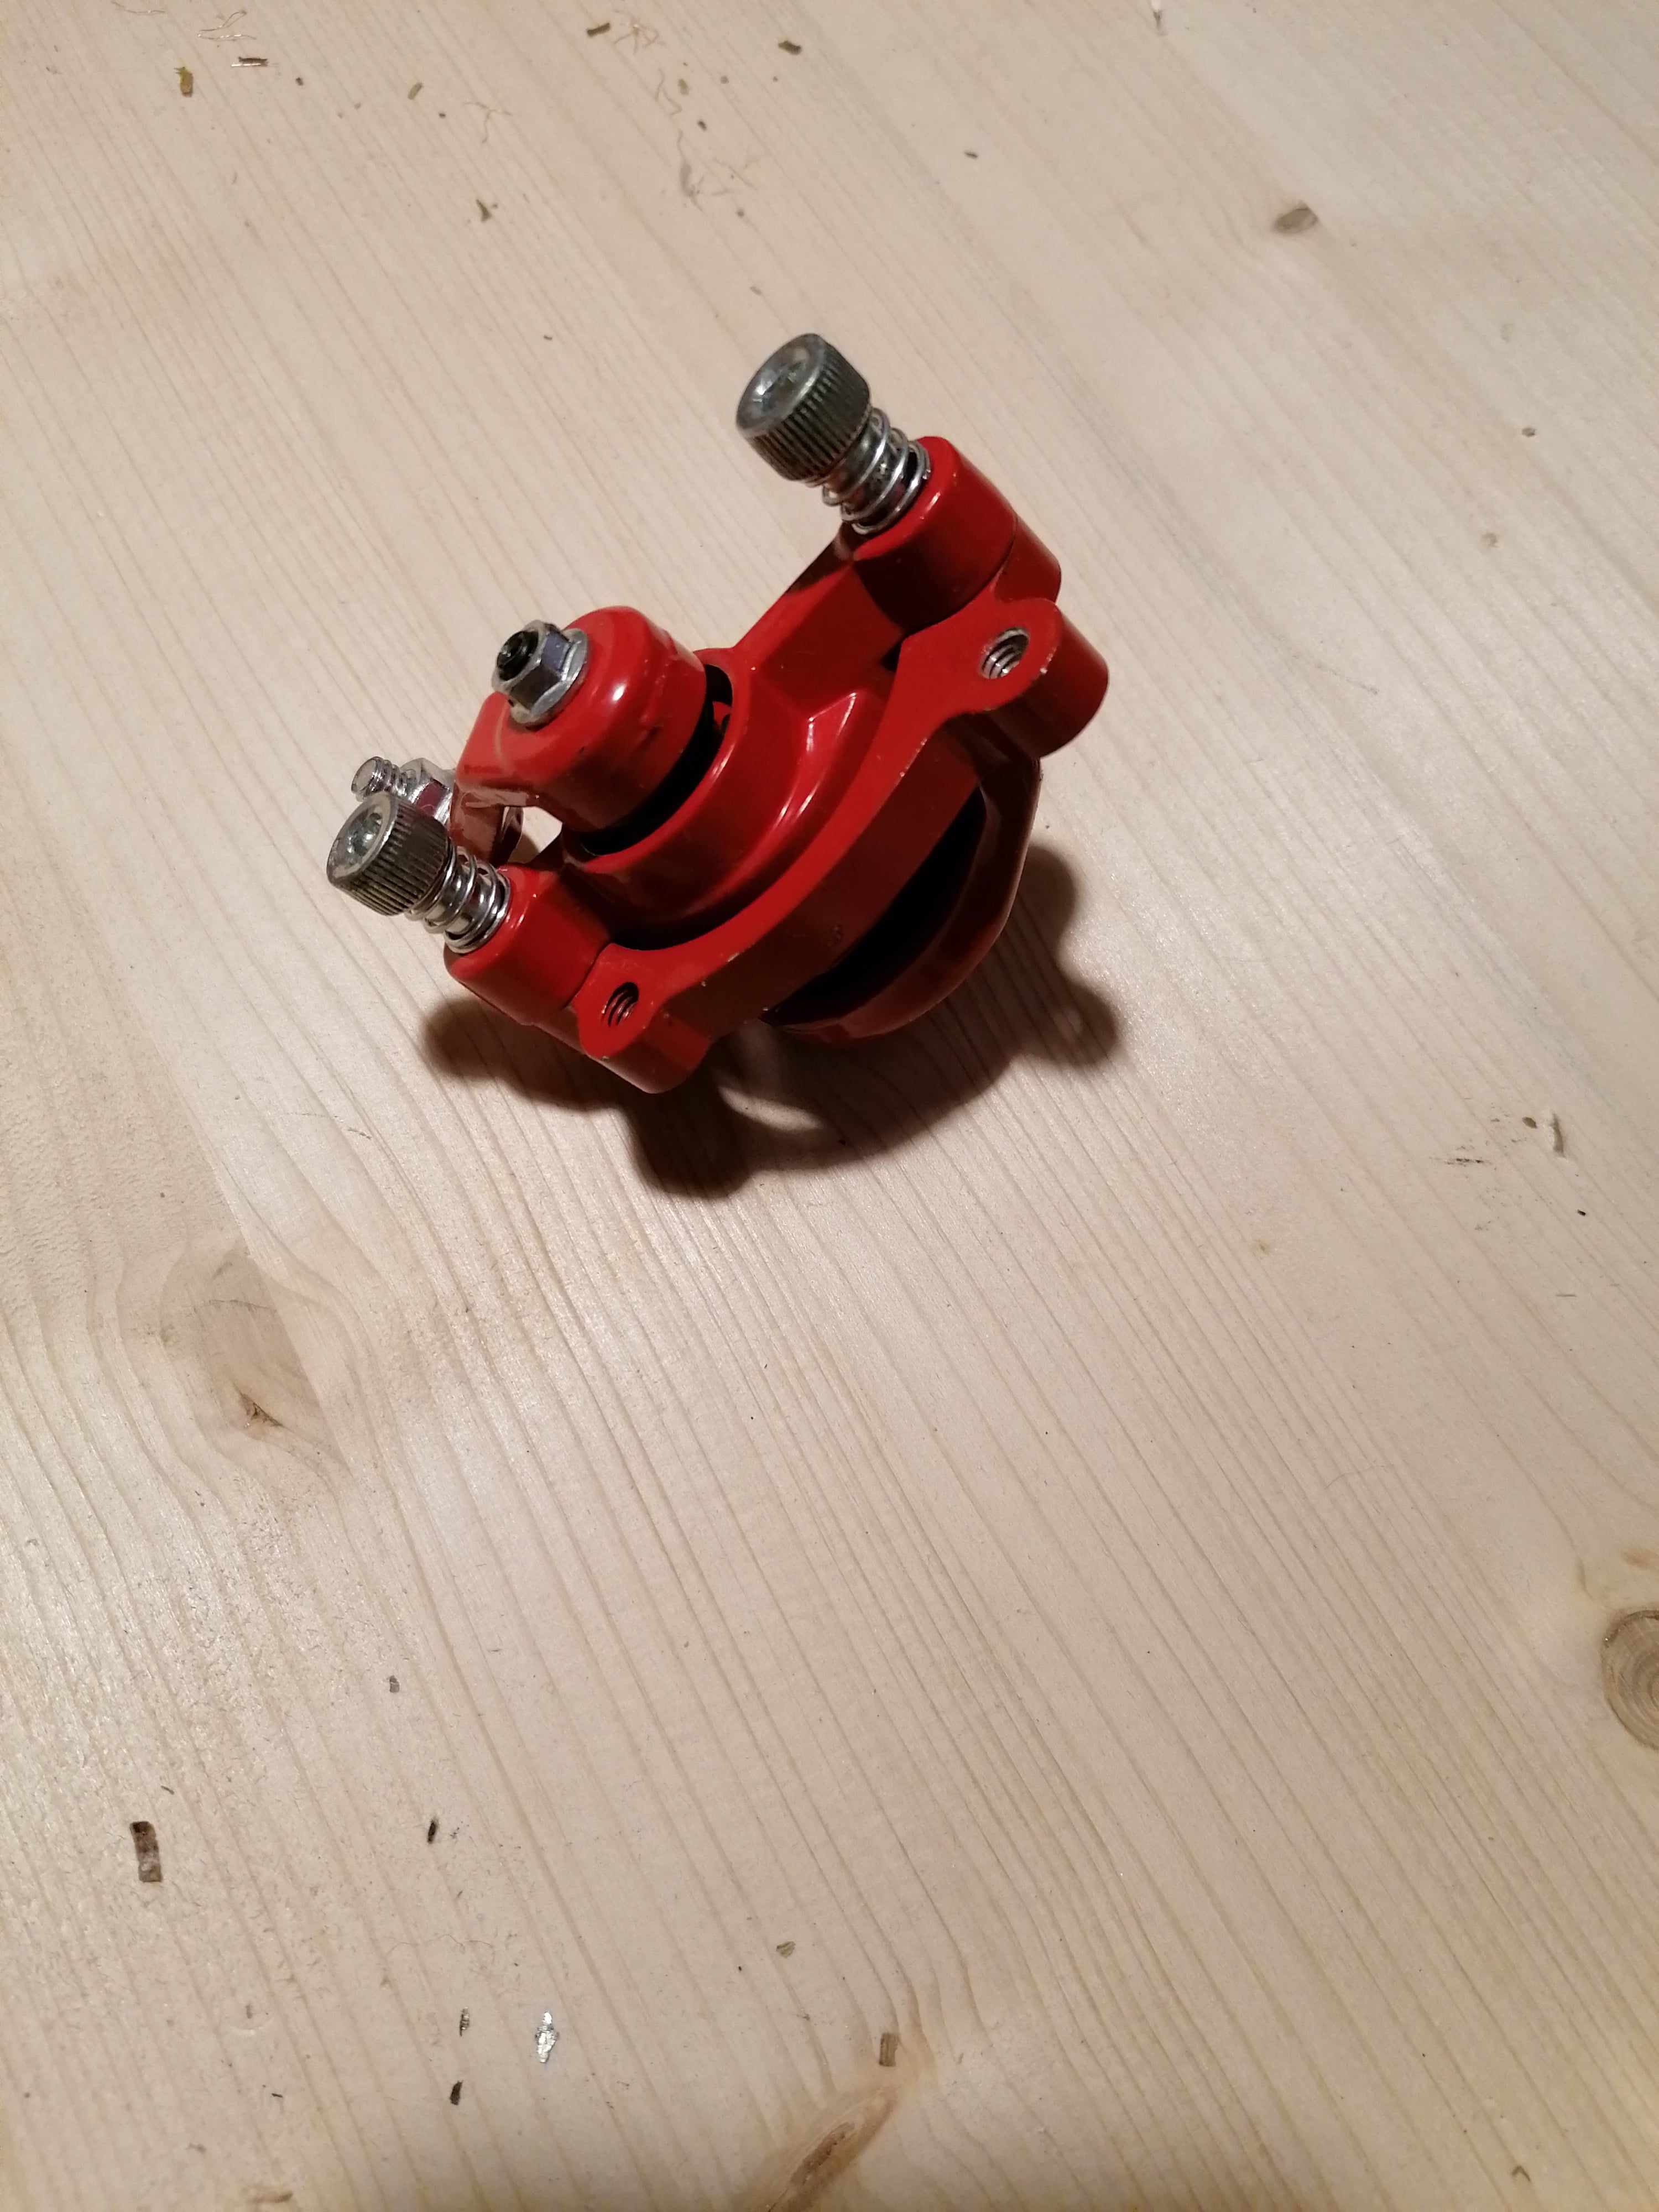
\includegraphics[width=0.3\textwidth]{bremssattel.jpg}}
    \hfill
    \caption{Bremssatz für den Laboraufbau}
\end{figure}